% Options for packages loaded elsewhere
\PassOptionsToPackage{unicode}{hyperref}
\PassOptionsToPackage{hyphens}{url}
%
\documentclass[
]{article}
\usepackage{amsmath,amssymb}
\usepackage{lmodern}
\usepackage{iftex}
\ifPDFTeX
  \usepackage[T1]{fontenc}
  \usepackage[utf8]{inputenc}
  \usepackage{textcomp} % provide euro and other symbols
\else % if luatex or xetex
  \usepackage{unicode-math}
  \defaultfontfeatures{Scale=MatchLowercase}
  \defaultfontfeatures[\rmfamily]{Ligatures=TeX,Scale=1}
\fi
% Use upquote if available, for straight quotes in verbatim environments
\IfFileExists{upquote.sty}{\usepackage{upquote}}{}
\IfFileExists{microtype.sty}{% use microtype if available
  \usepackage[]{microtype}
  \UseMicrotypeSet[protrusion]{basicmath} % disable protrusion for tt fonts
}{}
\makeatletter
\@ifundefined{KOMAClassName}{% if non-KOMA class
  \IfFileExists{parskip.sty}{%
    \usepackage{parskip}
  }{% else
    \setlength{\parindent}{0pt}
    \setlength{\parskip}{6pt plus 2pt minus 1pt}}
}{% if KOMA class
  \KOMAoptions{parskip=half}}
\makeatother
\usepackage{xcolor}
\usepackage[margin=1in]{geometry}
\usepackage{color}
\usepackage{fancyvrb}
\newcommand{\VerbBar}{|}
\newcommand{\VERB}{\Verb[commandchars=\\\{\}]}
\DefineVerbatimEnvironment{Highlighting}{Verbatim}{commandchars=\\\{\}}
% Add ',fontsize=\small' for more characters per line
\usepackage{framed}
\definecolor{shadecolor}{RGB}{248,248,248}
\newenvironment{Shaded}{\begin{snugshade}}{\end{snugshade}}
\newcommand{\AlertTok}[1]{\textcolor[rgb]{0.94,0.16,0.16}{#1}}
\newcommand{\AnnotationTok}[1]{\textcolor[rgb]{0.56,0.35,0.01}{\textbf{\textit{#1}}}}
\newcommand{\AttributeTok}[1]{\textcolor[rgb]{0.77,0.63,0.00}{#1}}
\newcommand{\BaseNTok}[1]{\textcolor[rgb]{0.00,0.00,0.81}{#1}}
\newcommand{\BuiltInTok}[1]{#1}
\newcommand{\CharTok}[1]{\textcolor[rgb]{0.31,0.60,0.02}{#1}}
\newcommand{\CommentTok}[1]{\textcolor[rgb]{0.56,0.35,0.01}{\textit{#1}}}
\newcommand{\CommentVarTok}[1]{\textcolor[rgb]{0.56,0.35,0.01}{\textbf{\textit{#1}}}}
\newcommand{\ConstantTok}[1]{\textcolor[rgb]{0.00,0.00,0.00}{#1}}
\newcommand{\ControlFlowTok}[1]{\textcolor[rgb]{0.13,0.29,0.53}{\textbf{#1}}}
\newcommand{\DataTypeTok}[1]{\textcolor[rgb]{0.13,0.29,0.53}{#1}}
\newcommand{\DecValTok}[1]{\textcolor[rgb]{0.00,0.00,0.81}{#1}}
\newcommand{\DocumentationTok}[1]{\textcolor[rgb]{0.56,0.35,0.01}{\textbf{\textit{#1}}}}
\newcommand{\ErrorTok}[1]{\textcolor[rgb]{0.64,0.00,0.00}{\textbf{#1}}}
\newcommand{\ExtensionTok}[1]{#1}
\newcommand{\FloatTok}[1]{\textcolor[rgb]{0.00,0.00,0.81}{#1}}
\newcommand{\FunctionTok}[1]{\textcolor[rgb]{0.00,0.00,0.00}{#1}}
\newcommand{\ImportTok}[1]{#1}
\newcommand{\InformationTok}[1]{\textcolor[rgb]{0.56,0.35,0.01}{\textbf{\textit{#1}}}}
\newcommand{\KeywordTok}[1]{\textcolor[rgb]{0.13,0.29,0.53}{\textbf{#1}}}
\newcommand{\NormalTok}[1]{#1}
\newcommand{\OperatorTok}[1]{\textcolor[rgb]{0.81,0.36,0.00}{\textbf{#1}}}
\newcommand{\OtherTok}[1]{\textcolor[rgb]{0.56,0.35,0.01}{#1}}
\newcommand{\PreprocessorTok}[1]{\textcolor[rgb]{0.56,0.35,0.01}{\textit{#1}}}
\newcommand{\RegionMarkerTok}[1]{#1}
\newcommand{\SpecialCharTok}[1]{\textcolor[rgb]{0.00,0.00,0.00}{#1}}
\newcommand{\SpecialStringTok}[1]{\textcolor[rgb]{0.31,0.60,0.02}{#1}}
\newcommand{\StringTok}[1]{\textcolor[rgb]{0.31,0.60,0.02}{#1}}
\newcommand{\VariableTok}[1]{\textcolor[rgb]{0.00,0.00,0.00}{#1}}
\newcommand{\VerbatimStringTok}[1]{\textcolor[rgb]{0.31,0.60,0.02}{#1}}
\newcommand{\WarningTok}[1]{\textcolor[rgb]{0.56,0.35,0.01}{\textbf{\textit{#1}}}}
\usepackage{graphicx}
\makeatletter
\def\maxwidth{\ifdim\Gin@nat@width>\linewidth\linewidth\else\Gin@nat@width\fi}
\def\maxheight{\ifdim\Gin@nat@height>\textheight\textheight\else\Gin@nat@height\fi}
\makeatother
% Scale images if necessary, so that they will not overflow the page
% margins by default, and it is still possible to overwrite the defaults
% using explicit options in \includegraphics[width, height, ...]{}
\setkeys{Gin}{width=\maxwidth,height=\maxheight,keepaspectratio}
% Set default figure placement to htbp
\makeatletter
\def\fps@figure{htbp}
\makeatother
\setlength{\emergencystretch}{3em} % prevent overfull lines
\providecommand{\tightlist}{%
  \setlength{\itemsep}{0pt}\setlength{\parskip}{0pt}}
\setcounter{secnumdepth}{-\maxdimen} % remove section numbering
\ifLuaTeX
  \usepackage{selnolig}  % disable illegal ligatures
\fi
\IfFileExists{bookmark.sty}{\usepackage{bookmark}}{\usepackage{hyperref}}
\IfFileExists{xurl.sty}{\usepackage{xurl}}{} % add URL line breaks if available
\urlstyle{same} % disable monospaced font for URLs
\hypersetup{
  pdftitle={Final Project},
  pdfauthor={Annie Lin},
  hidelinks,
  pdfcreator={LaTeX via pandoc}}

\title{Final Project}
\author{Annie Lin}
\date{2022-12-16}

\begin{document}
\maketitle

\hypertarget{project-proposal}{%
\subsection{Project Proposal}\label{project-proposal}}

There are many websites that can convert convert ICD-9 code into ICD-10
code (and vice versa), but they can only convert one code at a time,
which consumed me a lot of time when I did my BST210 regression project.
Thus, I want to use R to convert a set of ICD codes (as many as you
want) all at once.

For the 2nd part of this project, I will use data from Kaggle to build a
regression model to predict opioids overdose. Because back in Taiwan, I
was an anesthesiologist. In our daily practice, to treat patients' pain,
opioids (such as morphine) are often used. However, opioids are very
easily to be addictive to. Once these drugs are used overdose (very
likely for those drug abusers), they would not only put people into
sleep but suppress their breath, heart rate, and blood pressure -- but
people cannot react because they are deeply sedated! In the end, they
are usually found dead. To prevent these tragedies, if we can predict
people potentially with higher possibility of opioids overdose, we may
avoid using (or use less) these highly addictive drugs on them and adopt
other alternative treatment or medications.

\#\#Part 1 Data Wrangling \#\#Introduction

My ICD codes files are from
\href{https://www.nber.org/research/data/icd-9-cm-and-icd-10-cm-and-icd-10-pcs-crosswalk-or-general-equivalence-mappings}{here}.

\begin{verbatim}
## [1] 23912
\end{verbatim}

\begin{verbatim}
##   icd9cm icd10cm flags approximate no_map combination scenario choice_list
## 1     10    A000     0           0      0           0        0           0
## 2     11    A001     0           0      0           0        0           0
## 3     19    A009     0           0      0           0        0           0
## 4     20   A0100 10000           1      0           0        0           0
## 5     21    A011     0           0      0           0        0           0
## 6     22    A012     0           0      0           0        0           0
\end{verbatim}

There are 23912 codes in this file, whereas the ICD-9 and ICD-10 codes
are not in the correct form. Take the first row for example, there is no
ICD-9 code = 10, instead, it should be 001.0, while the corresponding
ICD-10 code = A00.0, rather than A000.

\begin{Shaded}
\begin{Highlighting}[]
\NormalTok{knitr}\SpecialCharTok{::}\FunctionTok{include\_graphics}\NormalTok{(}\FunctionTok{file.path}\NormalTok{(img\_path,}\StringTok{"icd.png"}\NormalTok{))}
\end{Highlighting}
\end{Shaded}

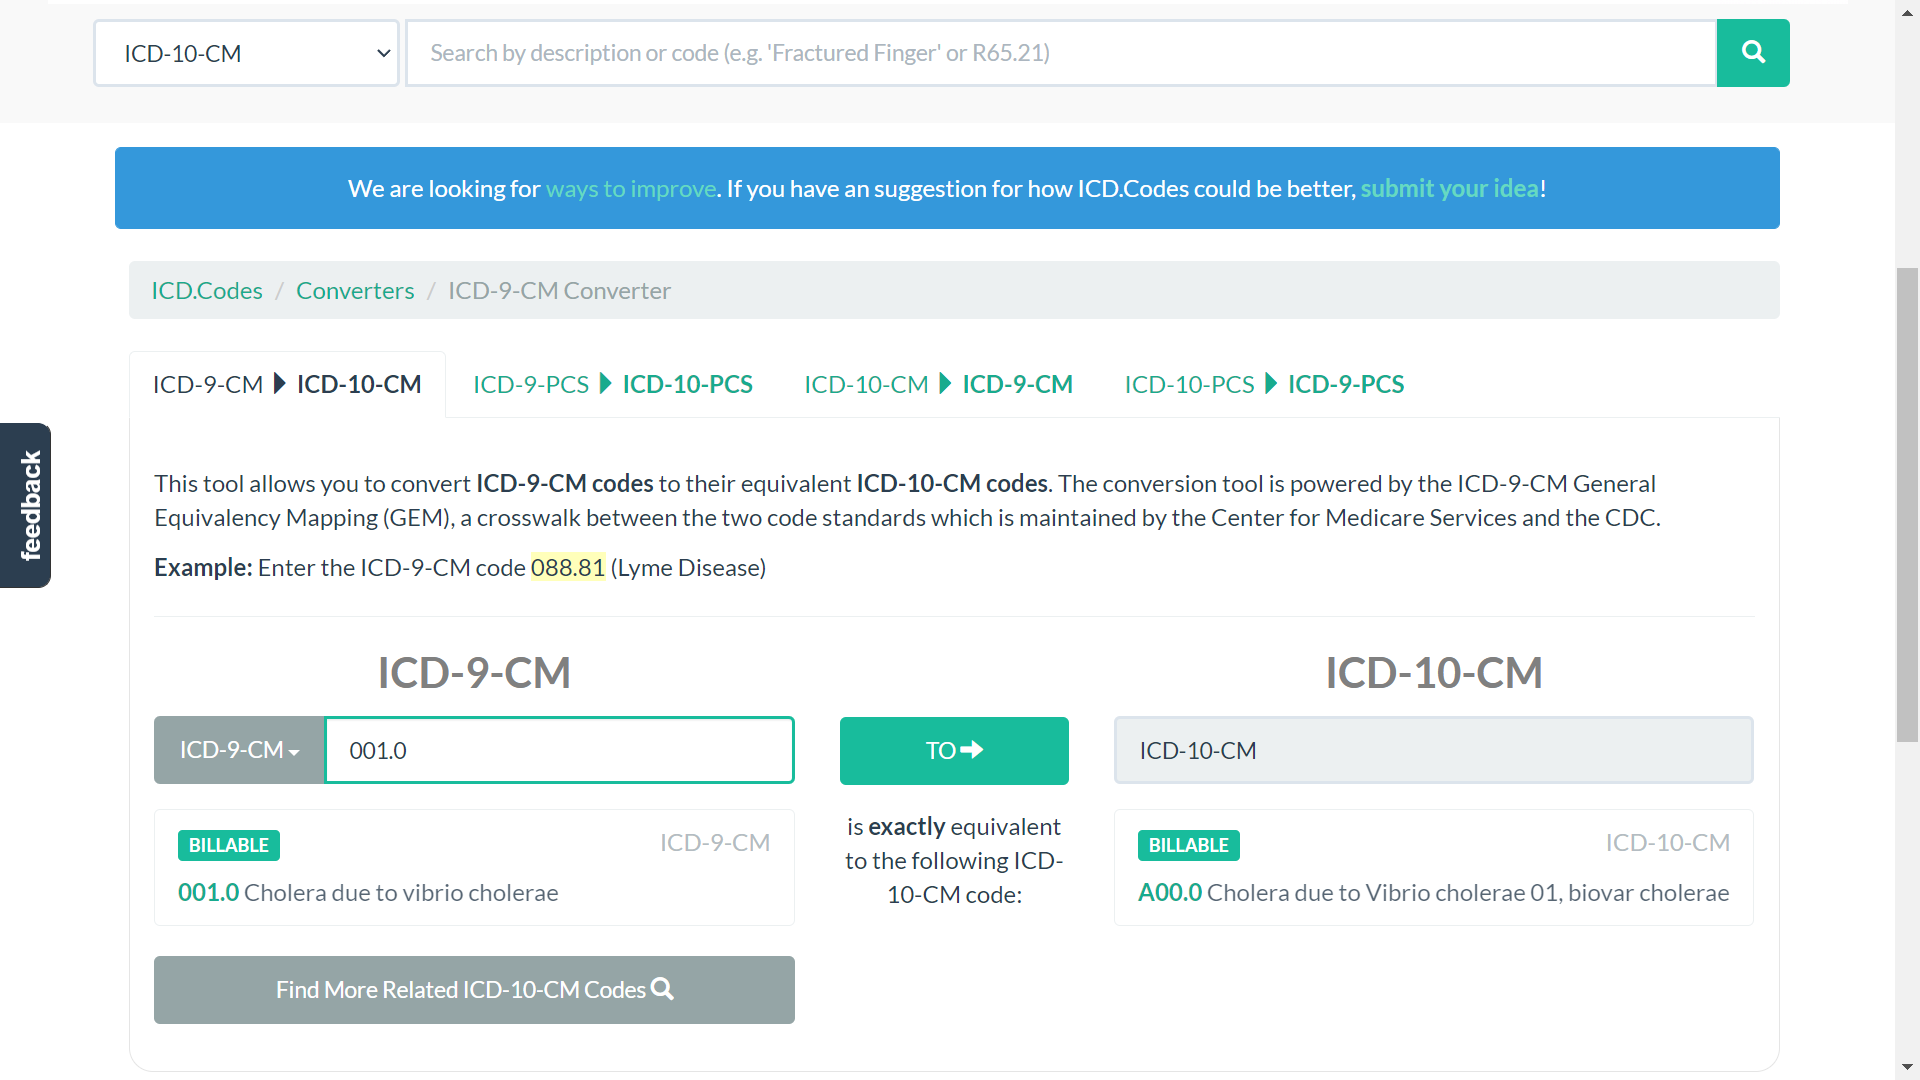
\includegraphics[width=26.67in]{img/icd}

Because of this error, there are identical ICD-9 codes in the file that
actually should be different and correspond to different ICD-10 codes.
Take ICD-9 = 320 in this file for example:

\begin{Shaded}
\begin{Highlighting}[]
\NormalTok{knitr}\SpecialCharTok{::}\FunctionTok{include\_graphics}\NormalTok{(}\FunctionTok{file.path}\NormalTok{(img\_path,}\StringTok{"icd 320a.png"}\NormalTok{))}
\end{Highlighting}
\end{Shaded}

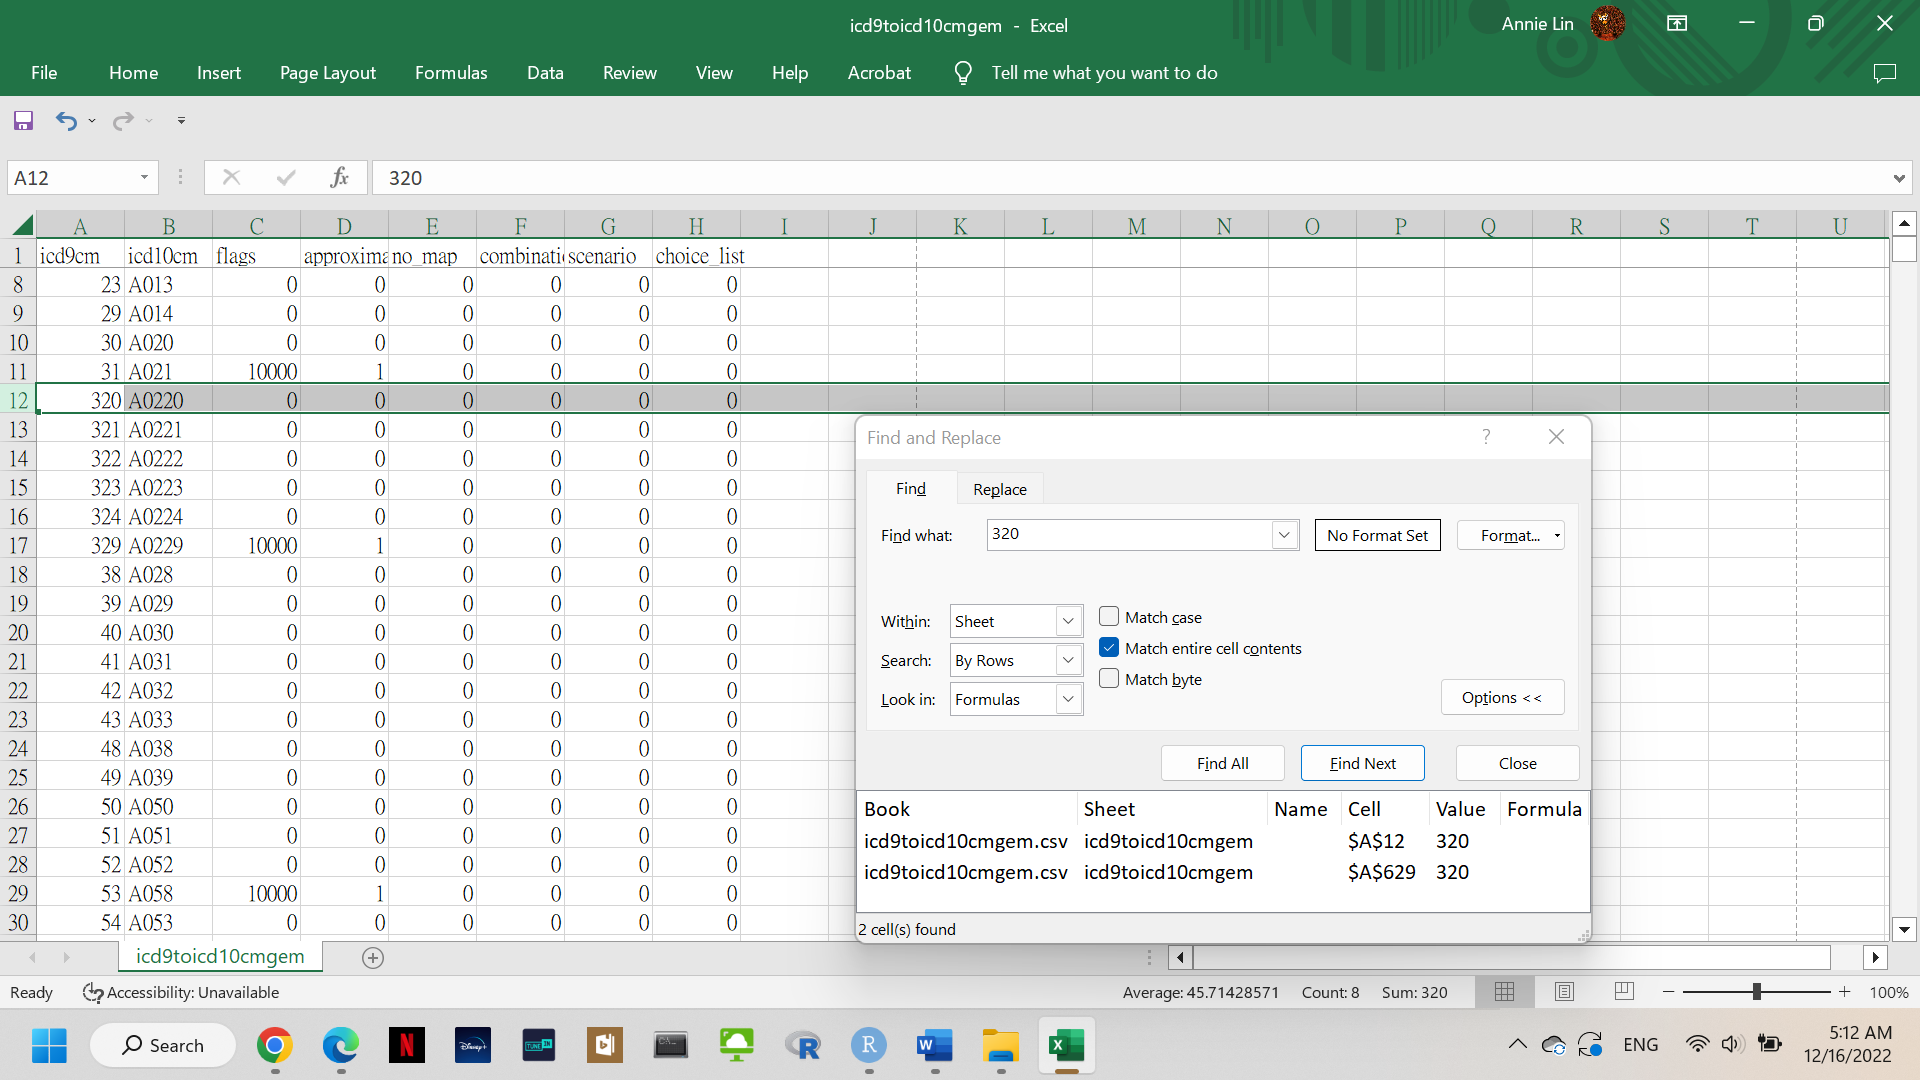
\includegraphics[width=26.67in]{img/icd 320a}

\begin{Shaded}
\begin{Highlighting}[]
\NormalTok{knitr}\SpecialCharTok{::}\FunctionTok{include\_graphics}\NormalTok{(}\FunctionTok{file.path}\NormalTok{(img\_path,}\StringTok{"icd 320b.png"}\NormalTok{))}
\end{Highlighting}
\end{Shaded}

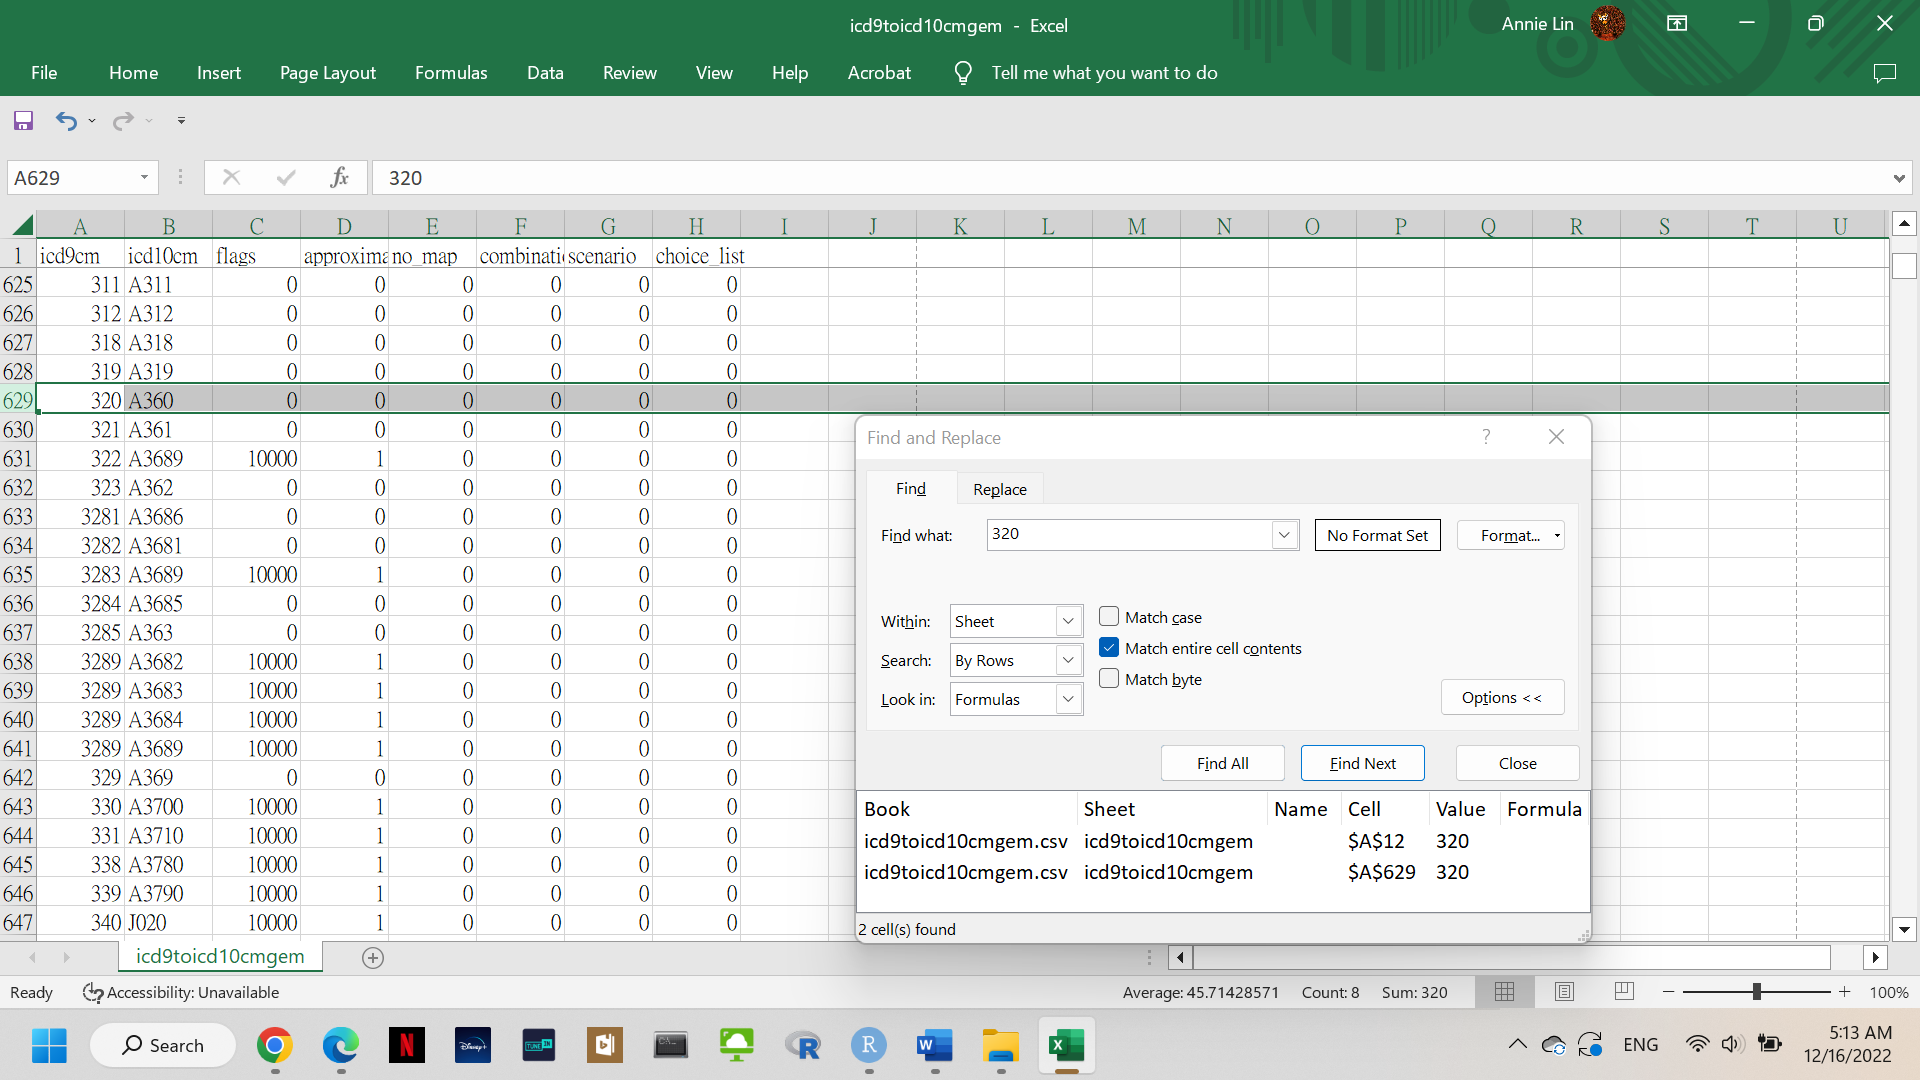
\includegraphics[width=26.67in]{img/icd 320b}

These 320s should be 003.20 and 032.0, while the corresponding ICD-10
codes are A02.20 (not A0220) and A36.0 (not A360):

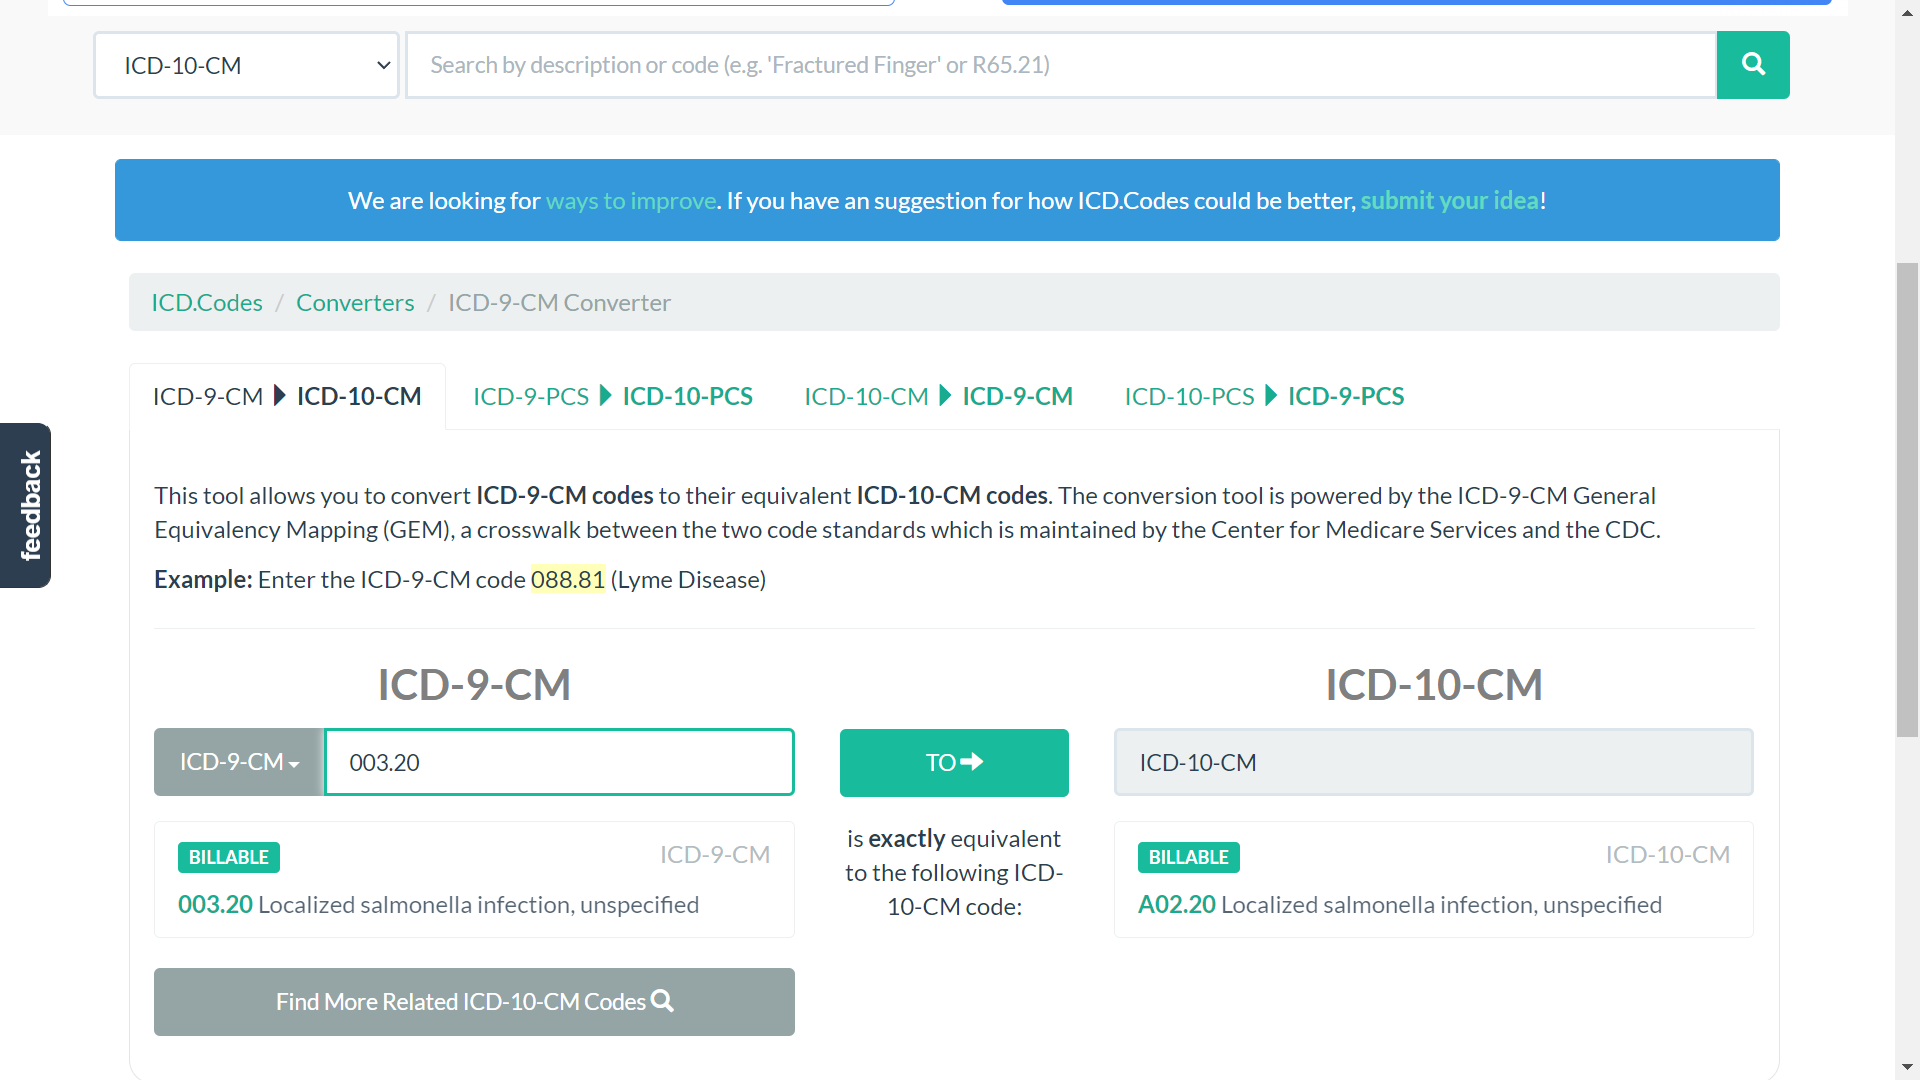
\includegraphics[width=0.5\linewidth]{img/icd 320 1}
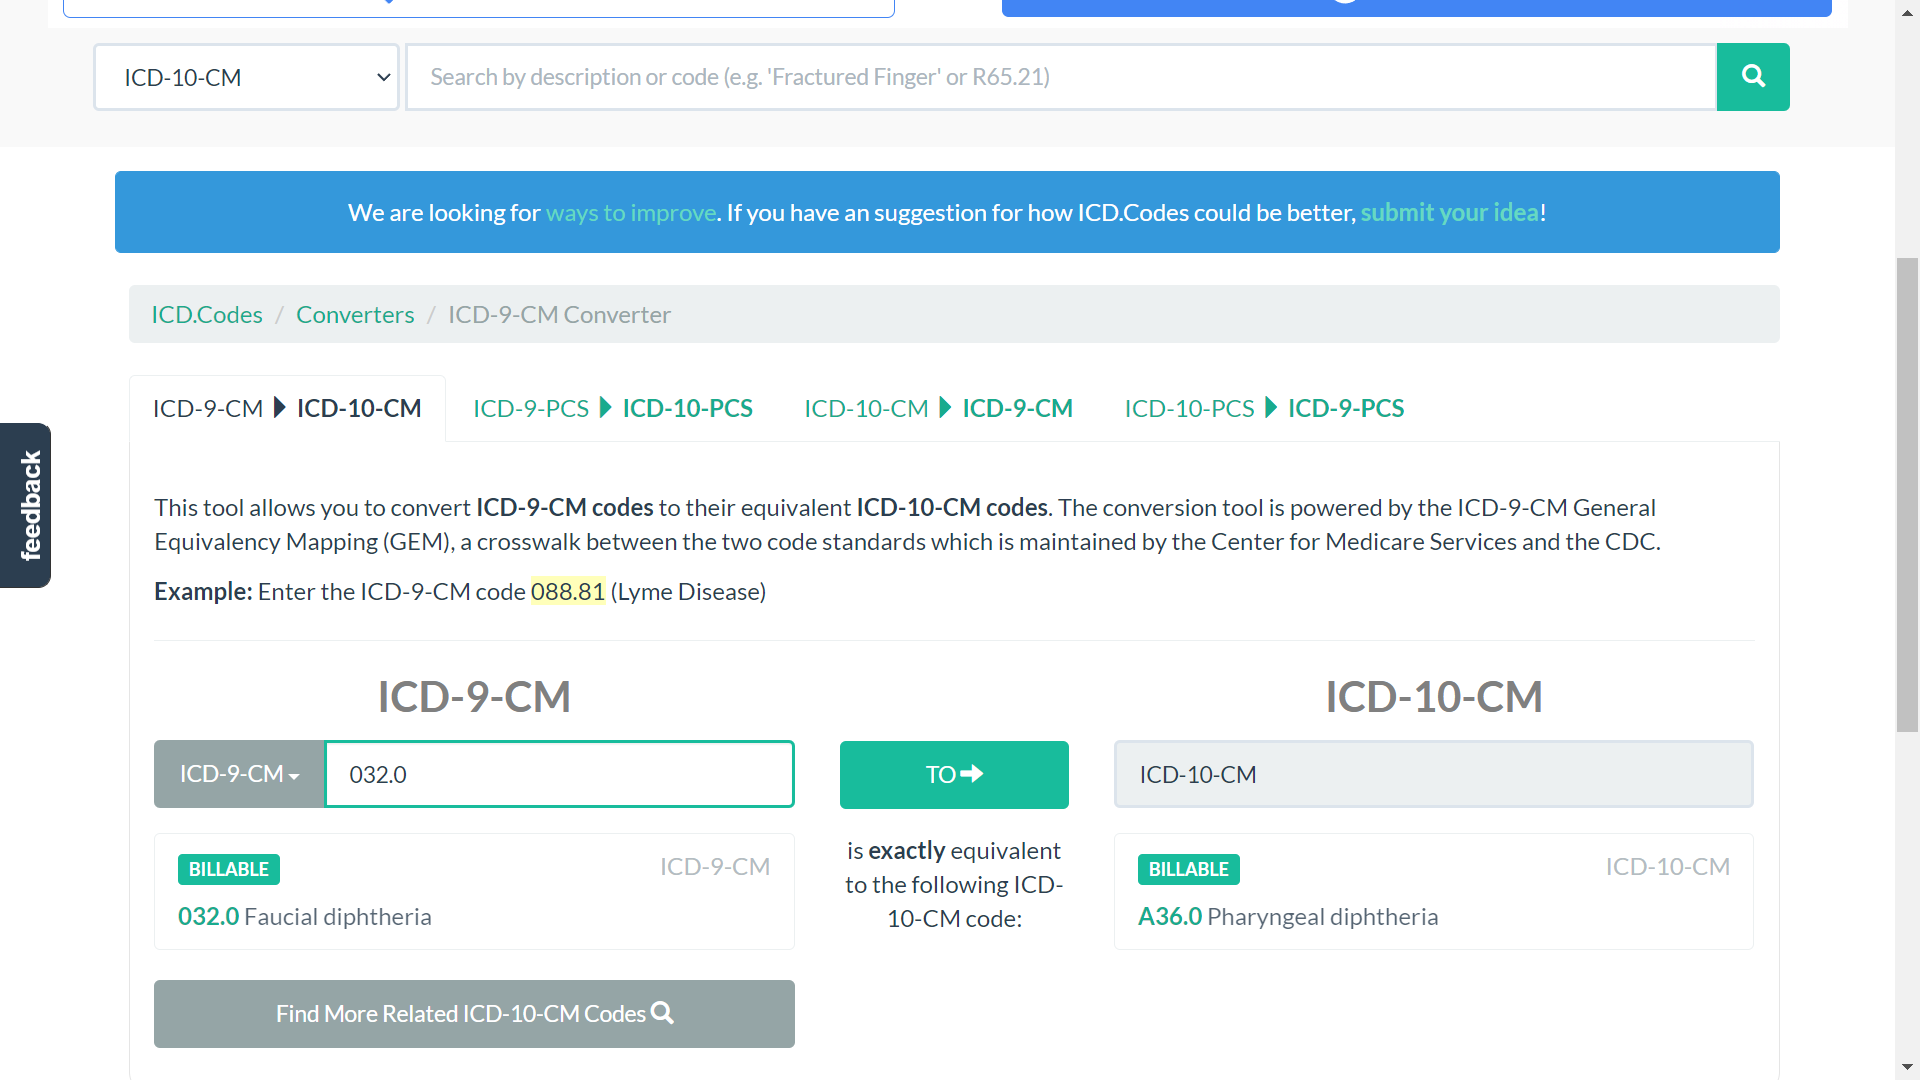
\includegraphics[width=0.5\linewidth]{img/icd 320 2}

Now you may find out that (1) in the correct ICD-codes, there should be
3 numbers or 1 alphabet with 2 numbers before the decimal; (2) for ICD-9
codes, we may need to add 1 zero or 2 zeros to some of the original
codes in our file.

Thus, after checking with the correct codes, I found out that in our
file: (1) for the first 1-81 ICD-9 codes, we need to add ``00'' before
the original number, and then add ``.'' after the 3rd number; (2) for
the first 82-1211 ICD-9 codes, we need to add ``0'' before the original
number, and then add ``.'' after the 3rd number; (3) for the rest
1212-23912 ICD-9 codes, we need to add ``.'' after the 3rd number; (4)
for all the ICD-10 codes, we just need to add ``.'' after the 3rd
number.

So let's start data wrangling!

\begin{verbatim}
## [1] "001.0" "001.1" "001.9" "002.0" "002.1" "002.2"
\end{verbatim}

\begin{verbatim}
## [1] "099.54" "099.55" "099.56" "099.59" "099.8"  "099.9"
\end{verbatim}

\begin{verbatim}
## [1] "100.0"  "100.81" "100.89" "100.9"  "101."   "101."
\end{verbatim}

\begin{verbatim}
## [1] "A00.0"  "A00.1"  "A00.9"  "A01.00" "A01.1"  "A01.2"
\end{verbatim}

\begin{verbatim}
##   icd9cm icd10cm flags approximate no_map combination scenario choice_list
## 1     10    A000     0           0      0           0        0           0
## 2     11    A001     0           0      0           0        0           0
## 3     19    A009     0           0      0           0        0           0
## 4     20   A0100 10000           1      0           0        0           0
## 5     21    A011     0           0      0           0        0           0
## 6     22    A012     0           0      0           0        0           0
##   icd9cm_n icd10cm_n
## 1    001.0     A00.0
## 2    001.1     A00.1
## 3    001.9     A00.9
## 4    002.0    A01.00
## 5    002.1     A01.1
## 6    002.2     A01.2
\end{verbatim}

And never forget those not-matching ones. We know that either in ICD-9
or ICD-10, there should be digits. If it's no digits, it might be ``NA''
or ``No data'' or something similar.

\begin{verbatim}
## [1] 0
\end{verbatim}

\begin{verbatim}
## [1] 425
\end{verbatim}

\begin{verbatim}
##   [1] "NoD.x" "NoD.x" "NoD.x" "NoD.x" "NoD.x" "NoD.x" "NoD.x" "NoD.x" "NoD.x"
##  [10] "NoD.x" "NoD.x" "NoD.x" "NoD.x" "NoD.x" "NoD.x" "NoD.x" "NoD.x" "NoD.x"
##  [19] "NoD.x" "NoD.x" "NoD.x" "NoD.x" "NoD.x" "NoD.x" "NoD.x" "NoD.x" "NoD.x"
##  [28] "NoD.x" "NoD.x" "NoD.x" "NoD.x" "NoD.x" "NoD.x" "NoD.x" "NoD.x" "NoD.x"
##  [37] "NoD.x" "NoD.x" "NoD.x" "NoD.x" "NoD.x" "NoD.x" "NoD.x" "NoD.x" "NoD.x"
##  [46] "NoD.x" "NoD.x" "NoD.x" "NoD.x" "NoD.x" "NoD.x" "NoD.x" "NoD.x" "NoD.x"
##  [55] "NoD.x" "NoD.x" "NoD.x" "NoD.x" "NoD.x" "NoD.x" "NoD.x" "NoD.x" "NoD.x"
##  [64] "NoD.x" "NoD.x" "NoD.x" "NoD.x" "NoD.x" "NoD.x" "NoD.x" "NoD.x" "NoD.x"
##  [73] "NoD.x" "NoD.x" "NoD.x" "NoD.x" "NoD.x" "NoD.x" "NoD.x" "NoD.x" "NoD.x"
##  [82] "NoD.x" "NoD.x" "NoD.x" "NoD.x" "NoD.x" "NoD.x" "NoD.x" "NoD.x" "NoD.x"
##  [91] "NoD.x" "NoD.x" "NoD.x" "NoD.x" "NoD.x" "NoD.x" "NoD.x" "NoD.x" "NoD.x"
## [100] "NoD.x" "NoD.x" "NoD.x" "NoD.x" "NoD.x" "NoD.x" "NoD.x" "NoD.x" "NoD.x"
## [109] "NoD.x" "NoD.x" "NoD.x" "NoD.x" "NoD.x" "NoD.x" "NoD.x" "NoD.x" "NoD.x"
## [118] "NoD.x" "NoD.x" "NoD.x" "NoD.x" "NoD.x" "NoD.x" "NoD.x" "NoD.x" "NoD.x"
## [127] "NoD.x" "NoD.x" "NoD.x" "NoD.x" "NoD.x" "NoD.x" "NoD.x" "NoD.x" "NoD.x"
## [136] "NoD.x" "NoD.x" "NoD.x" "NoD.x" "NoD.x" "NoD.x" "NoD.x" "NoD.x" "NoD.x"
## [145] "NoD.x" "NoD.x" "NoD.x" "NoD.x" "NoD.x" "NoD.x" "NoD.x" "NoD.x" "NoD.x"
## [154] "NoD.x" "NoD.x" "NoD.x" "NoD.x" "NoD.x" "NoD.x" "NoD.x" "NoD.x" "NoD.x"
## [163] "NoD.x" "NoD.x" "NoD.x" "NoD.x" "NoD.x" "NoD.x" "NoD.x" "NoD.x" "NoD.x"
## [172] "NoD.x" "NoD.x" "NoD.x" "NoD.x" "NoD.x" "NoD.x" "NoD.x" "NoD.x" "NoD.x"
## [181] "NoD.x" "NoD.x" "NoD.x" "NoD.x" "NoD.x" "NoD.x" "NoD.x" "NoD.x" "NoD.x"
## [190] "NoD.x" "NoD.x" "NoD.x" "NoD.x" "NoD.x" "NoD.x" "NoD.x" "NoD.x" "NoD.x"
## [199] "NoD.x" "NoD.x" "NoD.x" "NoD.x" "NoD.x" "NoD.x" "NoD.x" "NoD.x" "NoD.x"
## [208] "NoD.x" "NoD.x" "NoD.x" "NoD.x" "NoD.x" "NoD.x" "NoD.x" "NoD.x" "NoD.x"
## [217] "NoD.x" "NoD.x" "NoD.x" "NoD.x" "NoD.x" "NoD.x" "NoD.x" "NoD.x" "NoD.x"
## [226] "NoD.x" "NoD.x" "NoD.x" "NoD.x" "NoD.x" "NoD.x" "NoD.x" "NoD.x" "NoD.x"
## [235] "NoD.x" "NoD.x" "NoD.x" "NoD.x" "NoD.x" "NoD.x" "NoD.x" "NoD.x" "NoD.x"
## [244] "NoD.x" "NoD.x" "NoD.x" "NoD.x" "NoD.x" "NoD.x" "NoD.x" "NoD.x" "NoD.x"
## [253] "NoD.x" "NoD.x" "NoD.x" "NoD.x" "NoD.x" "NoD.x" "NoD.x" "NoD.x" "NoD.x"
## [262] "NoD.x" "NoD.x" "NoD.x" "NoD.x" "NoD.x" "NoD.x" "NoD.x" "NoD.x" "NoD.x"
## [271] "NoD.x" "NoD.x" "NoD.x" "NoD.x" "NoD.x" "NoD.x" "NoD.x" "NoD.x" "NoD.x"
## [280] "NoD.x" "NoD.x" "NoD.x" "NoD.x" "NoD.x" "NoD.x" "NoD.x" "NoD.x" "NoD.x"
## [289] "NoD.x" "NoD.x" "NoD.x" "NoD.x" "NoD.x" "NoD.x" "NoD.x" "NoD.x" "NoD.x"
## [298] "NoD.x" "NoD.x" "NoD.x" "NoD.x" "NoD.x" "NoD.x" "NoD.x" "NoD.x" "NoD.x"
## [307] "NoD.x" "NoD.x" "NoD.x" "NoD.x" "NoD.x" "NoD.x" "NoD.x" "NoD.x" "NoD.x"
## [316] "NoD.x" "NoD.x" "NoD.x" "NoD.x" "NoD.x" "NoD.x" "NoD.x" "NoD.x" "NoD.x"
## [325] "NoD.x" "NoD.x" "NoD.x" "NoD.x" "NoD.x" "NoD.x" "NoD.x" "NoD.x" "NoD.x"
## [334] "NoD.x" "NoD.x" "NoD.x" "NoD.x" "NoD.x" "NoD.x" "NoD.x" "NoD.x" "NoD.x"
## [343] "NoD.x" "NoD.x" "NoD.x" "NoD.x" "NoD.x" "NoD.x" "NoD.x" "NoD.x" "NoD.x"
## [352] "NoD.x" "NoD.x" "NoD.x" "NoD.x" "NoD.x" "NoD.x" "NoD.x" "NoD.x" "NoD.x"
## [361] "NoD.x" "NoD.x" "NoD.x" "NoD.x" "NoD.x" "NoD.x" "NoD.x" "NoD.x" "NoD.x"
## [370] "NoD.x" "NoD.x" "NoD.x" "NoD.x" "NoD.x" "NoD.x" "NoD.x" "NoD.x" "NoD.x"
## [379] "NoD.x" "NoD.x" "NoD.x" "NoD.x" "NoD.x" "NoD.x" "NoD.x" "NoD.x" "NoD.x"
## [388] "NoD.x" "NoD.x" "NoD.x" "NoD.x" "NoD.x" "NoD.x" "NoD.x" "NoD.x" "NoD.x"
## [397] "NoD.x" "NoD.x" "NoD.x" "NoD.x" "NoD.x" "NoD.x" "NoD.x" "NoD.x" "NoD.x"
## [406] "NoD.x" "NoD.x" "NoD.x" "NoD.x" "NoD.x" "NoD.x" "NoD.x" "NoD.x" "NoD.x"
## [415] "NoD.x" "NoD.x" "NoD.x" "NoD.x" "NoD.x" "NoD.x" "NoD.x" "NoD.x" "NoD.x"
## [424] "NoD.x" "NoD.x"
\end{verbatim}

So there is no NA in our corrected ICD-9 codes (GOOD!), but there are
425 ``NoD.x'' in the corrected ICD-10 codes. Let's replace it with NA.

Now let's add the disease description into our new dataset.

\begin{verbatim}
## [1] "CODE"                                 
## [2] "LONG.DESCRIPTION..VALID.ICD.9.FY2023."
\end{verbatim}

\begin{verbatim}
##   CODE LONG.DESCRIPTION..VALID.ICD.9.FY2023.
## 1 0010        Cholera due to vibrio cholerae
## 2 0011 Cholera due to vibrio cholerae el tor
## 3 0019                  Cholera, unspecified
## 4 0020                         Typhoid fever
## 5 0021                   Paratyphoid fever A
## 6 0022                   Paratyphoid fever B
\end{verbatim}

\begin{verbatim}
## [1] "character"
\end{verbatim}

\begin{verbatim}
## [1] 13521
\end{verbatim}

\begin{verbatim}
##    CODE                                  SHORT.DESCRIPTION
## 1  A000 Cholera due to Vibrio cholerae 01, biovar cholerae
## 2  A001    Cholera due to Vibrio cholerae 01, biovar eltor
## 3  A009                               Cholera, unspecified
## 4 A0100                         Typhoid fever, unspecified
## 5 A0101                                 Typhoid meningitis
## 6 A0102               Typhoid fever with heart involvement
##                                     LONG.DESCRIPTION
## 1 Cholera due to Vibrio cholerae 01, biovar cholerae
## 2    Cholera due to Vibrio cholerae 01, biovar eltor
## 3                               Cholera, unspecified
## 4                         Typhoid fever, unspecified
## 5                                 Typhoid meningitis
## 6               Typhoid fever with heart involvement
\end{verbatim}

\begin{verbatim}
## [1] FALSE
\end{verbatim}

\begin{verbatim}
##      CODE                                            SHORT.DESCRIPTION
## 41  A0472   Enterocolitis d/t Clostridium difficile, not spcf as recur
## 46   A052               Foodborne Clostridium perfringens intoxication
## 123 A1883                  Tuberculosis of digestive tract organs, NEC
## 177  A288    Oth zoonotic bacterial diseases, not elsewhere classified
## 189  A312     Dissem mycobacterium avium-intracellulare complex (DMAC)
## 217 A3710 Whooping cough due to Bordetella parapertussis w/o pneumonia
##                                                           LONG.DESCRIPTION
## 41  Enterocolitis due to Clostridium difficile, not specified as recurrent
## 46    Foodborne Clostridium perfringens [Clostridium welchii] intoxication
## 123       Tuberculosis of digestive tract organs, not elsewhere classified
## 177  Other specified zoonotic bacterial diseases, not elsewhere classified
## 189         Disseminated mycobacterium avium-intracellulare complex (DMAC)
## 217       Whooping cough due to Bordetella parapertussis without pneumonia
\end{verbatim}

\begin{verbatim}
## [1] 72836
\end{verbatim}

There are two disease descriptions in the icd\_cm\_10d file, I will use
the more detailed one (the long description). And in these two files,
the codes also should be corrected just like above. After correction, we
can join the tables.

\begin{verbatim}
## [1] "001.0" "001.1" "001.9" "002.0" "002.1" "002.2"
\end{verbatim}

\begin{verbatim}
##   CODE LONG.DESCRIPTION..VALID.ICD.9.FY2023. icd9cm_n
## 1 0010        Cholera due to vibrio cholerae    001.0
## 2 0011 Cholera due to vibrio cholerae el tor    001.1
## 3 0019                  Cholera, unspecified    001.9
## 4 0020                         Typhoid fever    002.0
## 5 0021                   Paratyphoid fever A    002.1
## 6 0022                   Paratyphoid fever B    002.2
\end{verbatim}

\begin{verbatim}
## [1] "A00.0"  "A00.1"  "A00.9"  "A01.00" "A01.01" "A01.02"
\end{verbatim}

\begin{verbatim}
##    CODE                                  SHORT.DESCRIPTION
## 1  A000 Cholera due to Vibrio cholerae 01, biovar cholerae
## 2  A001    Cholera due to Vibrio cholerae 01, biovar eltor
## 3  A009                               Cholera, unspecified
## 4 A0100                         Typhoid fever, unspecified
## 5 A0101                                 Typhoid meningitis
## 6 A0102               Typhoid fever with heart involvement
##                                     LONG.DESCRIPTION icd10cm_n
## 1 Cholera due to Vibrio cholerae 01, biovar cholerae     A00.0
## 2    Cholera due to Vibrio cholerae 01, biovar eltor     A00.1
## 3                               Cholera, unspecified     A00.9
## 4                         Typhoid fever, unspecified    A01.00
## 5                                 Typhoid meningitis    A01.01
## 6               Typhoid fever with heart involvement    A01.02
\end{verbatim}

\begin{verbatim}
##  [1] "icd9cm"      "icd10cm"     "flags"       "approximate" "no_map"     
##  [6] "combination" "scenario"    "choice_list" "icd9cm_n"    "icd10cm_n"
\end{verbatim}

\begin{verbatim}
## [1] "CODE"                                 
## [2] "LONG.DESCRIPTION..VALID.ICD.9.FY2023."
## [3] "icd9cm_n"
\end{verbatim}

\begin{verbatim}
##   icd9cm icd10cm flags approximate no_map combination scenario choice_list
## 1     10    A000     0           0      0           0        0           0
## 2     11    A001     0           0      0           0        0           0
## 3     19    A009     0           0      0           0        0           0
## 4     20   A0100 10000           1      0           0        0           0
## 5     21    A011     0           0      0           0        0           0
## 6     22    A012     0           0      0           0        0           0
##   icd9cm_n icd10cm_n CODE LONG.DESCRIPTION..VALID.ICD.9.FY2023.
## 1    001.0     A00.0 0010        Cholera due to vibrio cholerae
## 2    001.1     A00.1 0011 Cholera due to vibrio cholerae el tor
## 3    001.9     A00.9 0019                  Cholera, unspecified
## 4    002.0    A01.00 0020                         Typhoid fever
## 5    002.1     A01.1 0021                   Paratyphoid fever A
## 6    002.2     A01.2 0022                   Paratyphoid fever B
\end{verbatim}

\begin{verbatim}
##   icd9cm icd10cm flags approximate no_map combination scenario choice_list
## 1     10    A000     0           0      0           0        0           0
## 2     11    A001     0           0      0           0        0           0
## 3     19    A009     0           0      0           0        0           0
## 4     20   A0100 10000           1      0           0        0           0
## 5     21    A011     0           0      0           0        0           0
## 6     22    A012     0           0      0           0        0           0
##   icd9cm_n icd10cm_n CODE.x                      ICD9 Description CODE.y
## 1    001.0     A00.0   0010        Cholera due to vibrio cholerae   A000
## 2    001.1     A00.1   0011 Cholera due to vibrio cholerae el tor   A001
## 3    001.9     A00.9   0019                  Cholera, unspecified   A009
## 4    002.0    A01.00   0020                         Typhoid fever  A0100
## 5    002.1     A01.1   0021                   Paratyphoid fever A   A011
## 6    002.2     A01.2   0022                   Paratyphoid fever B   A012
##                                    SHORT.DESCRIPTION
## 1 Cholera due to Vibrio cholerae 01, biovar cholerae
## 2    Cholera due to Vibrio cholerae 01, biovar eltor
## 3                               Cholera, unspecified
## 4                         Typhoid fever, unspecified
## 5                                Paratyphoid fever A
## 6                                Paratyphoid fever B
##                                     LONG.DESCRIPTION
## 1 Cholera due to Vibrio cholerae 01, biovar cholerae
## 2    Cholera due to Vibrio cholerae 01, biovar eltor
## 3                               Cholera, unspecified
## 4                         Typhoid fever, unspecified
## 5                                Paratyphoid fever A
## 6                                Paratyphoid fever B
\end{verbatim}

\begin{verbatim}
##  [1] "icd9cm"            "icd10cm"           "flags"            
##  [4] "approximate"       "no_map"            "combination"      
##  [7] "scenario"          "choice_list"       "icd9cm_n"         
## [10] "icd10cm_n"         "CODE.x"            "ICD9 Description" 
## [13] "CODE.y"            "SHORT.DESCRIPTION" "LONG.DESCRIPTION"
\end{verbatim}

\begin{verbatim}
##  [1] "icd9cm"            "icd10cm"           "flags"            
##  [4] "approximate"       "no_map"            "combination"      
##  [7] "scenario"          "choice_list"       "icd9cm_n"         
## [10] "icd10cm_n"         "CODE.x"            "ICD9 Description" 
## [13] "CODE.y"            "SHORT.DESCRIPTION" "ICD10 Description"
\end{verbatim}

Lastly, we need to add some warning signs because sometimes ICD-9 codes
cannot exactly match with the ICD-10 codes. Notice those flags? When the
flag = 0, it means we can find the exact ICD-10 codes; when the flag =
10000, it means we can only find the most similar meaning ICD-10 codes;
when the flag = 11000, sadly there's no such ICD-10 codes. This is our
last step of data wrangling!

\begin{verbatim}
##   icd9cm icd10cm flags icd9cm_n icd10cm_n                      ICD9 Description
## 1     10    A000     0    001.0     A00.0        Cholera due to vibrio cholerae
## 2     11    A001     0    001.1     A00.1 Cholera due to vibrio cholerae el tor
## 3     19    A009     0    001.9     A00.9                  Cholera, unspecified
## 4     20   A0100 10000    002.0    A01.00                         Typhoid fever
## 5     21    A011     0    002.1     A01.1                   Paratyphoid fever A
## 6     22    A012     0    002.2     A01.2                   Paratyphoid fever B
##                                    ICD10 Description              matching
## 1 Cholera due to Vibrio cholerae 01, biovar cholerae      Exactly matching
## 2    Cholera due to Vibrio cholerae 01, biovar eltor      Exactly matching
## 3                               Cholera, unspecified      Exactly matching
## 4                         Typhoid fever, unspecified Approxiately matching
## 5                                Paratyphoid fever A      Exactly matching
## 6                                Paratyphoid fever B      Exactly matching
\end{verbatim}

\begin{verbatim}
##   icd9cm_n icd10cm_n                      ICD9 Description
## 1    001.0     A00.0        Cholera due to vibrio cholerae
## 2    001.1     A00.1 Cholera due to vibrio cholerae el tor
## 3    001.9     A00.9                  Cholera, unspecified
## 4    002.0    A01.00                         Typhoid fever
## 5    002.1     A01.1                   Paratyphoid fever A
## 6    002.2     A01.2                   Paratyphoid fever B
##                                    ICD10 Description              matching
## 1 Cholera due to Vibrio cholerae 01, biovar cholerae      Exactly matching
## 2    Cholera due to Vibrio cholerae 01, biovar eltor      Exactly matching
## 3                               Cholera, unspecified      Exactly matching
## 4                         Typhoid fever, unspecified Approxiately matching
## 5                                Paratyphoid fever A      Exactly matching
## 6                                Paratyphoid fever B      Exactly matching
\end{verbatim}

\hypertarget{results}{%
\subsection{Results}\label{results}}

Finally, we can start to search the matching ICD-10 codes! For example,
if I want to convert ICD-9 = ``E93.00'',``003.1'',``032.0'':

\begin{Shaded}
\begin{Highlighting}[]
\NormalTok{icd\_cm\_final }\SpecialCharTok{|\textgreater{}}
  \FunctionTok{filter}\NormalTok{(icd9cm\_n }\SpecialCharTok{\%in\%} \FunctionTok{c}\NormalTok{(}\StringTok{"E93.00"}\NormalTok{,}\StringTok{"003.1"}\NormalTok{,}\StringTok{"032.0"}\NormalTok{)) }\SpecialCharTok{|\textgreater{}} 
  \FunctionTok{summarise}\NormalTok{(}\AttributeTok{icd9 =}\NormalTok{ icd9cm\_n, }\AttributeTok{icd10 =}\NormalTok{ icd10cm\_n, }\AttributeTok{footnote =}\NormalTok{ matching)}
\end{Highlighting}
\end{Shaded}

\begin{verbatim}
##     icd9 icd10              footnote
## 1  003.1 A02.1 Approxiately matching
## 2  032.0 A36.0      Exactly matching
## 3 E93.00  <NA>           No matching
\end{verbatim}

We can find the corresponding ICD-10 codes along with their matching
extent in the summarize (footnote). And we can directly copy the
corresponding ICD-10 codes into our word files or slides by using codes
below:

\begin{Shaded}
\begin{Highlighting}[]
\NormalTok{exp1 }\OtherTok{=}\NormalTok{ icd\_cm\_final }\SpecialCharTok{|\textgreater{}}
  \FunctionTok{filter}\NormalTok{(icd9cm\_n }\SpecialCharTok{\%in\%} \FunctionTok{c}\NormalTok{(}\StringTok{"E93.00"}\NormalTok{,}\StringTok{"003.1"}\NormalTok{,}\StringTok{"032.0"}\NormalTok{)) }\SpecialCharTok{|\textgreater{}} 
  \FunctionTok{summarise}\NormalTok{(}\AttributeTok{icd9 =}\NormalTok{ icd9cm\_n, }\AttributeTok{icd10 =}\NormalTok{ icd10cm\_n, }\AttributeTok{footnote =}\NormalTok{ matching) }\SpecialCharTok{|\textgreater{}}
  \FunctionTok{pull}\NormalTok{(icd10)}

\NormalTok{exp1 }\SpecialCharTok{|\textgreater{}} 
  \FunctionTok{paste}\NormalTok{(}\AttributeTok{collapse =} \StringTok{" "}\NormalTok{) }\SpecialCharTok{|\textgreater{}}
  \FunctionTok{str\_replace\_all}\NormalTok{(}\StringTok{" "}\NormalTok{, }\StringTok{", "}\NormalTok{)    }
\end{Highlighting}
\end{Shaded}

\begin{verbatim}
## [1] "A02.1, A36.0, NA"
\end{verbatim}

By using the codes below, we can directly copy a number of ICD codes
from word files and paste them into '' '' and search!! No need to spend
time to further separate them with '' ``!

\begin{Shaded}
\begin{Highlighting}[]
\NormalTok{exp2 }\OtherTok{=} \FunctionTok{c}\NormalTok{(}\StringTok{"E93.00, 003.1, 032.0"}\NormalTok{)  }
\NormalTok{e2 }\OtherTok{=} \FunctionTok{unlist}\NormalTok{(}\FunctionTok{str\_split}\NormalTok{(exp2, }\StringTok{", "}\NormalTok{))}

\NormalTok{icd\_cm\_final }\SpecialCharTok{|\textgreater{}}
  \FunctionTok{filter}\NormalTok{(icd9cm\_n }\SpecialCharTok{\%in\%} \FunctionTok{c}\NormalTok{(e2[}\DecValTok{1}\SpecialCharTok{:}\FunctionTok{length}\NormalTok{(e2)])) }\SpecialCharTok{|\textgreater{}} 
  \FunctionTok{summarise}\NormalTok{(}\AttributeTok{icd9 =}\NormalTok{ icd9cm\_n, }\AttributeTok{icd10 =}\NormalTok{ icd10cm\_n, }\AttributeTok{footnote =}\NormalTok{ matching) }\SpecialCharTok{|\textgreater{}}
  \FunctionTok{pull}\NormalTok{(icd10)     }
\end{Highlighting}
\end{Shaded}

\begin{verbatim}
## [1] "A02.1" "A36.0" NA
\end{verbatim}

This is what I want!

\#\#Part 2 Regression model

As mentioned above, I want to build a regression model to predict the
possibility of opioids overdose.

Firstly, the mean of opioids overdose rate is 8. I defined opioids
overdose rate \textgreater8 as more likely to have opioids overdose, and
\textless=8 as less likely, which becomes overdose\_p in the data.

Secondly, Using overdose\_p as outcome, putting all the possible
covariates into the model as our full model (logistic regression).

Though the performance of the full model is good (AIC= 417.32, AUC =
0.99), because there are many covariates related to finance, such as
thealthspend (total health spend) and totalrealhcspend (total real
hospital and clinics spend), considering collinearity and
simplicity/parsimony, stateid (state), totalrealhcspend (total health
spend), labor\_participation\_pct (labor or not), grad\_hs\_pct
(education), and cpi (consumer price index) are kept in my final model
(s\_model).

The performance of this final model is nice, with AIC: 551.68 and AUC =
0.9755.

\begin{Shaded}
\begin{Highlighting}[]
\NormalTok{op }\OtherTok{=} \FunctionTok{read.csv}\NormalTok{(}\StringTok{"c:}\SpecialCharTok{\textbackslash{}\textbackslash{}}\StringTok{Users}\SpecialCharTok{\textbackslash{}\textbackslash{}}\StringTok{user}\SpecialCharTok{\textbackslash{}\textbackslash{}}\StringTok{Downloads}\SpecialCharTok{\textbackslash{}\textbackslash{}}\StringTok{Opioid.csv"}\NormalTok{)}
\FunctionTok{head}\NormalTok{(op)}
\end{Highlighting}
\end{Shaded}

\begin{verbatim}
##     state stateid year t mcare_millions medicaid_spend_actual medicaidspending
## 1 Alabama       1 2000 0           3690               2719.15          2.7e+09
## 2 Alabama       1 2001 1           4065               2901.74          2.9e+09
## 3 Alabama       1 2002 2           4394               3115.61          3.1e+09
## 4 Alabama       1 2003 3           4756               3505.83          3.5e+09
## 5 Alabama       1 2004 4           5274               3664.08          3.7e+09
## 6 Alabama       1 2005 5           5698               3864.14          3.9e+09
##   thealthspend totalrealhcspend overdoses population overdose_rate
## 1         6410             9410        43    4500000         0.956
## 2         6970             9860        57    4500000         1.270
## 3         7510            10500        71    4500000         1.580
## 4         8260            11300        49    4500000         1.090
## 5         8940            12000        83    4500000         1.840
## 6         9560            12400        80    4600000         1.740
##   mdhhincomereal stategdpml realstategdp unemployment_pct
## 1          35424     119242     175097.8              4.6
## 2          35160     122449     173337.7              5.1
## 3          37603     127792     178858.3              5.9
## 4          37255     133739     182443.0              6.0
## 5          36629     146525     196107.7              5.7
## 6          37150     155970     202728.3              4.5
##   labor_participation_pct insured_pct grad_hs_pct is_manufacturing_state
## 1                    60.3        87.5        77.5                      1
## 2                    59.2        87.6        80.2                      1
## 3                    58.2        87.8        78.9                      1
## 4                    58.2        87.5        79.9                      1
## 5                    58.5        88.0        82.4                      1
## 6                    58.9        86.0        80.9                      1
##   post_recession   cpi
## 1              0 168.8
## 2              0 175.1
## 3              0 177.1
## 4              0 181.7
## 5              0 185.2
## 6              0 190.7
\end{verbatim}

\begin{Shaded}
\begin{Highlighting}[]
\FunctionTok{summary}\NormalTok{(op}\SpecialCharTok{$}\NormalTok{overdose\_rate)}
\end{Highlighting}
\end{Shaded}

\begin{verbatim}
##    Min. 1st Qu.  Median    Mean 3rd Qu.    Max. 
##   0.365   4.170   6.410   8.173  10.000  46.300
\end{verbatim}

\begin{Shaded}
\begin{Highlighting}[]
\NormalTok{op}\SpecialCharTok{$}\NormalTok{overdose\_p }\OtherTok{=} \FunctionTok{ifelse}\NormalTok{(op}\SpecialCharTok{$}\NormalTok{overdose\_rate }\SpecialCharTok{\textgreater{}}\DecValTok{8}\NormalTok{, }\DecValTok{1}\NormalTok{,}\DecValTok{0}\NormalTok{)}
\FunctionTok{names}\NormalTok{(op)}
\end{Highlighting}
\end{Shaded}

\begin{verbatim}
##  [1] "state"                   "stateid"                
##  [3] "year"                    "t"                      
##  [5] "mcare_millions"          "medicaid_spend_actual"  
##  [7] "medicaidspending"        "thealthspend"           
##  [9] "totalrealhcspend"        "overdoses"              
## [11] "population"              "overdose_rate"          
## [13] "mdhhincomereal"          "stategdpml"             
## [15] "realstategdp"            "unemployment_pct"       
## [17] "labor_participation_pct" "insured_pct"            
## [19] "grad_hs_pct"             "is_manufacturing_state" 
## [21] "post_recession"          "cpi"                    
## [23] "overdose_p"
\end{verbatim}

\begin{Shaded}
\begin{Highlighting}[]
\FunctionTok{library}\NormalTok{(ggplot2)}
\FunctionTok{library}\NormalTok{(tidyverse)}
\FunctionTok{library}\NormalTok{(caret)}
\FunctionTok{library}\NormalTok{(leaps)}
\FunctionTok{library}\NormalTok{(MASS)}
\FunctionTok{library}\NormalTok{(pROC)}
\FunctionTok{library}\NormalTok{(plotROC)}

\NormalTok{full\_model }\OtherTok{=} \FunctionTok{glm}\NormalTok{(overdose\_p }\SpecialCharTok{\textasciitilde{}}\NormalTok{ stateid }\SpecialCharTok{+}\NormalTok{ mcare\_millions }\SpecialCharTok{+}\NormalTok{ medicaid\_spend\_actual }\SpecialCharTok{+}\NormalTok{ medicaidspending }\SpecialCharTok{+}\NormalTok{ thealthspend }\SpecialCharTok{+}\NormalTok{ totalrealhcspend }\SpecialCharTok{+}\NormalTok{ mdhhincomereal }\SpecialCharTok{+}\NormalTok{ stategdpml }\SpecialCharTok{+}\NormalTok{ realstategdp }\SpecialCharTok{+}\NormalTok{ unemployment\_pct }\SpecialCharTok{+}\NormalTok{ labor\_participation\_pct }\SpecialCharTok{+}\NormalTok{ insured\_pct }\SpecialCharTok{+}\NormalTok{ grad\_hs\_pct }\SpecialCharTok{+}\NormalTok{ is\_manufacturing\_state }\SpecialCharTok{+}\NormalTok{ post\_recession }\SpecialCharTok{+}\NormalTok{ cpi , }\AttributeTok{data =}\NormalTok{ op, }\AttributeTok{family =} \StringTok{"binomial"}\NormalTok{)}

\FunctionTok{summary}\NormalTok{(full\_model)}
\end{Highlighting}
\end{Shaded}

\begin{verbatim}
## 
## Call:
## glm(formula = overdose_p ~ stateid + mcare_millions + medicaid_spend_actual + 
##     medicaidspending + thealthspend + totalrealhcspend + mdhhincomereal + 
##     stategdpml + realstategdp + unemployment_pct + labor_participation_pct + 
##     insured_pct + grad_hs_pct + is_manufacturing_state + post_recession + 
##     cpi, family = "binomial", data = op)
## 
## Deviance Residuals: 
##     Min       1Q   Median       3Q      Max  
## -2.3053  -0.6741  -0.2413   0.6604   2.9909  
## 
## Coefficients:
##                           Estimate Std. Error z value Pr(>|z|)    
## (Intercept)              6.233e+00  4.451e+00   1.400 0.161436    
## stateid                  5.309e-02  6.542e-03   8.115 4.85e-16 ***
## mcare_millions           4.370e-03  3.166e-03   1.380 0.167549    
## medicaid_spend_actual    4.592e-03  3.222e-03   1.425 0.154030    
## medicaidspending        -2.700e-10  6.913e-10  -0.391 0.696140    
## thealthspend            -3.373e-03  3.120e-03  -1.081 0.279562    
## totalrealhcspend        -7.857e-04  2.282e-04  -3.444 0.000573 ***
## mdhhincomereal           1.561e-04  1.841e-05   8.475  < 2e-16 ***
## stategdpml              -4.130e-05  1.415e-05  -2.919 0.003512 ** 
## realstategdp             2.916e-05  1.237e-05   2.357 0.018433 *  
## unemployment_pct         2.240e-01  7.051e-02   3.177 0.001487 ** 
## labor_participation_pct -1.519e-01  4.046e-02  -3.754 0.000174 ***
## insured_pct             -4.179e-02  2.916e-02  -1.433 0.151847    
## grad_hs_pct             -7.048e-02  4.330e-02  -1.628 0.103591    
## is_manufacturing_state  -7.297e-01  2.409e-01  -3.029 0.002455 ** 
## post_recession          -8.966e-01  4.494e-01  -1.995 0.046036 *  
## cpi                      1.496e-02  1.156e-02   1.294 0.195680    
## ---
## Signif. codes:  0 '***' 0.001 '**' 0.01 '*' 0.05 '.' 0.1 ' ' 1
## 
## (Dispersion parameter for binomial family taken to be 1)
## 
##     Null deviance: 1286.74  on 968  degrees of freedom
## Residual deviance:  833.02  on 952  degrees of freedom
## AIC: 867.02
## 
## Number of Fisher Scoring iterations: 6
\end{verbatim}

\begin{Shaded}
\begin{Highlighting}[]
\NormalTok{roc\_curve\_f }\OtherTok{=} \FunctionTok{roc}\NormalTok{(op}\SpecialCharTok{$}\NormalTok{overdose\_p ,}\FunctionTok{predict}\NormalTok{(full\_model, }\AttributeTok{type =} \FunctionTok{c}\NormalTok{(}\StringTok{"response"}\NormalTok{)))}
\NormalTok{roc\_curve\_f}\SpecialCharTok{$}\NormalTok{auc}
\end{Highlighting}
\end{Shaded}

\begin{verbatim}
## Area under the curve: 0.8729
\end{verbatim}

\begin{Shaded}
\begin{Highlighting}[]
\FunctionTok{ggplot}\NormalTok{(op, }\FunctionTok{aes}\NormalTok{(}\AttributeTok{m =} \FunctionTok{predict}\NormalTok{(full\_model, }\AttributeTok{type =} \FunctionTok{c}\NormalTok{(}\StringTok{"response"}\NormalTok{)), }\AttributeTok{d =}\NormalTok{ overdose\_p))}\SpecialCharTok{+} \FunctionTok{geom\_roc}\NormalTok{(}\AttributeTok{n.cuts =} \DecValTok{0}\NormalTok{, }\AttributeTok{labels =}\NormalTok{ F, }\AttributeTok{col =} \StringTok{"blue"}\NormalTok{)}\SpecialCharTok{+} \FunctionTok{style\_roc}\NormalTok{(}\AttributeTok{theme =}\NormalTok{ theme\_grey) }\SpecialCharTok{+} \FunctionTok{ggtitle}\NormalTok{(}\StringTok{"ROC curve (AUC=0.99) by full model"}\NormalTok{)}
\end{Highlighting}
\end{Shaded}

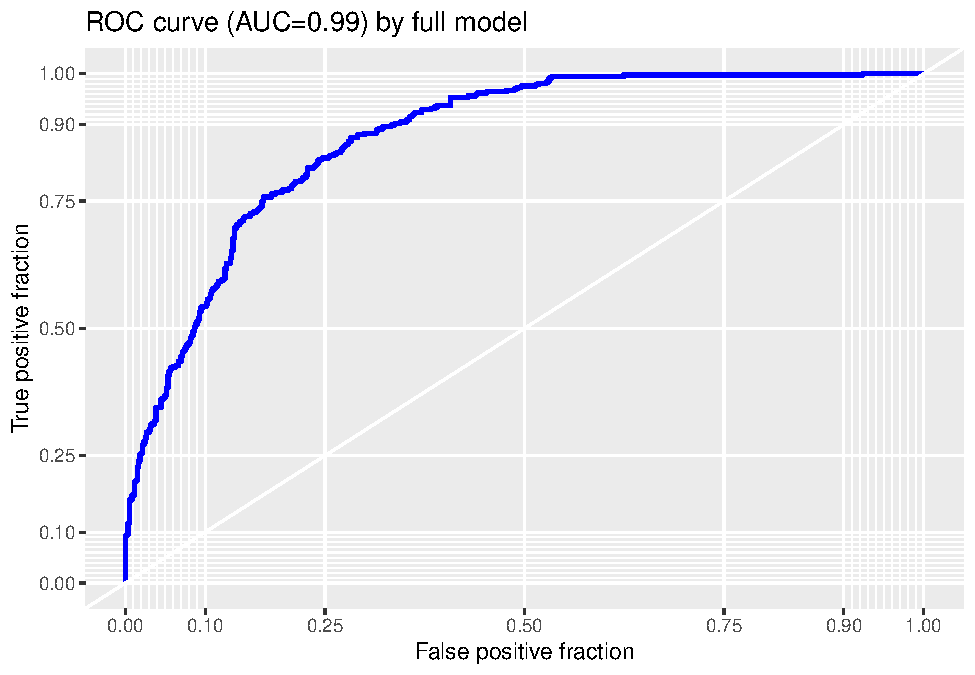
\includegraphics{Final-project_Annie-Lin-1_files/figure-latex/unnamed-chunk-15-1.pdf}

\begin{Shaded}
\begin{Highlighting}[]
\NormalTok{s\_model }\OtherTok{=} \FunctionTok{glm}\NormalTok{(}\AttributeTok{formula =}\NormalTok{ overdose\_p }\SpecialCharTok{\textasciitilde{}}\NormalTok{ stateid }\SpecialCharTok{+}\NormalTok{ totalrealhcspend }\SpecialCharTok{+}\NormalTok{ labor\_participation\_pct }\SpecialCharTok{+}
\NormalTok{                grad\_hs\_pct }\SpecialCharTok{+}\NormalTok{ cpi, }\AttributeTok{data =}\NormalTok{ op)}
\FunctionTok{summary}\NormalTok{(s\_model)}
\end{Highlighting}
\end{Shaded}

\begin{verbatim}
## 
## Call:
## glm(formula = overdose_p ~ stateid + totalrealhcspend + labor_participation_pct + 
##     grad_hs_pct + cpi, data = op)
## 
## Deviance Residuals: 
##      Min        1Q    Median        3Q       Max  
## -0.92288  -0.31954  -0.08052   0.35230   1.08393  
## 
## Coefficients:
##                           Estimate Std. Error t value Pr(>|t|)    
## (Intercept)             -1.089e+00  3.403e-01  -3.200  0.00142 ** 
## stateid                  5.956e-03  9.182e-04   6.486 1.40e-10 ***
## totalrealhcspend        -2.016e-06  6.207e-07  -3.247  0.00120 ** 
## labor_participation_pct -2.516e-02  4.541e-03  -5.541 3.87e-08 ***
## grad_hs_pct              1.663e-02  5.742e-03   2.896  0.00386 ** 
## cpi                      6.989e-03  7.577e-04   9.225  < 2e-16 ***
## ---
## Signif. codes:  0 '***' 0.001 '**' 0.01 '*' 0.05 '.' 0.1 ' ' 1
## 
## (Dispersion parameter for gaussian family taken to be 0.1744889)
## 
##     Null deviance: 228.24  on 968  degrees of freedom
## Residual deviance: 168.03  on 963  degrees of freedom
## AIC: 1066.1
## 
## Number of Fisher Scoring iterations: 2
\end{verbatim}

\begin{Shaded}
\begin{Highlighting}[]
\NormalTok{roc\_curve }\OtherTok{=} \FunctionTok{roc}\NormalTok{(op}\SpecialCharTok{$}\NormalTok{overdose\_p ,}\FunctionTok{predict}\NormalTok{(s\_model, }\AttributeTok{type =} \FunctionTok{c}\NormalTok{(}\StringTok{"response"}\NormalTok{)))}
\NormalTok{roc\_curve}\SpecialCharTok{$}\NormalTok{auc}
\end{Highlighting}
\end{Shaded}

\begin{verbatim}
## Area under the curve: 0.8079
\end{verbatim}

\begin{Shaded}
\begin{Highlighting}[]
\FunctionTok{ggplot}\NormalTok{(op, }\FunctionTok{aes}\NormalTok{(}\AttributeTok{m =} \FunctionTok{predict}\NormalTok{(s\_model, }\AttributeTok{type =} \FunctionTok{c}\NormalTok{(}\StringTok{"response"}\NormalTok{)), }\AttributeTok{d =}\NormalTok{ overdose\_p))}\SpecialCharTok{+} \FunctionTok{geom\_roc}\NormalTok{(}\AttributeTok{n.cuts =} \DecValTok{0}\NormalTok{, }\AttributeTok{labels =}\NormalTok{ F, }\AttributeTok{col =} \StringTok{"red"}\NormalTok{)}\SpecialCharTok{+} \FunctionTok{style\_roc}\NormalTok{(}\AttributeTok{theme =}\NormalTok{ theme\_grey) }\SpecialCharTok{+} \FunctionTok{ggtitle}\NormalTok{(}\StringTok{"ROC curve (AUC=0.98) by final model"}\NormalTok{)}
\end{Highlighting}
\end{Shaded}

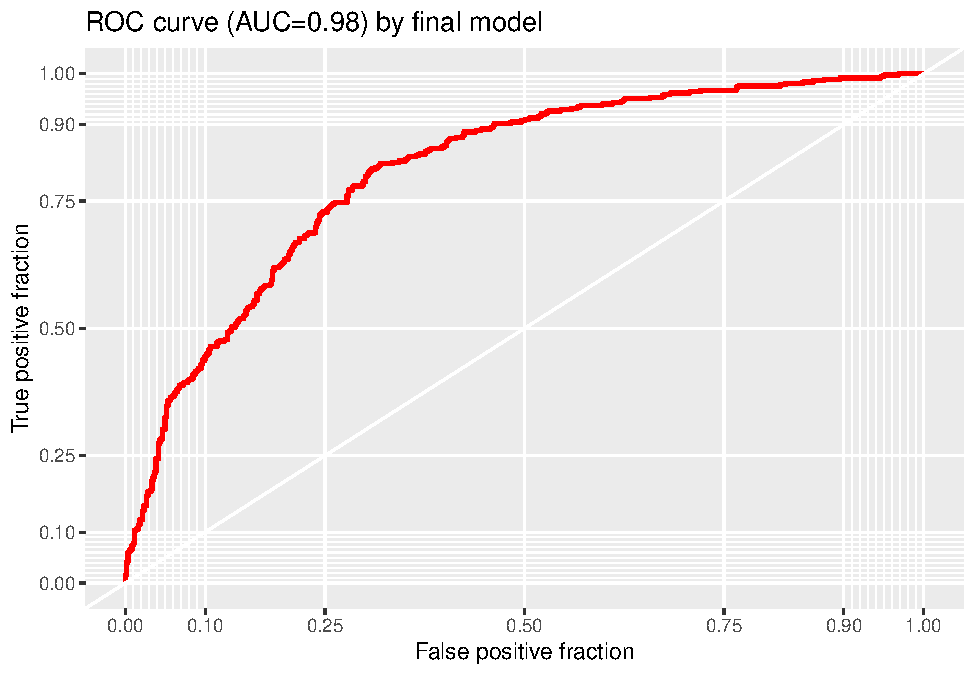
\includegraphics{Final-project_Annie-Lin-1_files/figure-latex/unnamed-chunk-15-2.pdf}

\#\#Conclusion

In part 1, I did data wrangling to convert ICD-9 to ICD-10. In part 2, I
built a logistic regression model to predict the possibility of opioids
overdose. I think both parts are quite successful. If I have more time,
I would like to apply machine learning skills in part 2.

\end{document}
